\documentclass{spbseu}


\title[]{Учебная практика}
\subtitle{<<Анализ социальных графов>>}
\titlegraphic{\begin{flushleft}\vspace{-1.5cm}\includegraphics[width=8cm,height=4.5cm]{images/title}\end{flushleft}}
\date{}
\institute{СПбГЭУ}
\author[]{Бронников Егор}


\begin{document}

    % 1 слайд
	\begin{frame}
		\titlepage
	\end{frame}
	
    % 2 слайд
	\begin{frame}
		\tableofcontents
	\end{frame}
	
	\section{Введение}
    % 3 слайд
	\begin{frame}
		\frametitle{Введение}
		\tableofcontents[part=1, pausesections]
        Практическая работа посвящена построению эго-графов пользователей в социальной сети ВКонтакте, вычислению основных показателей сети и выделение пользователей в группы (сообщества).
		\begin{block}{Цель исследования}
            \justifying
            Приобретение навыков научно-исследовательской работы, посвящённой анализу эго-графов пользователей социальной сети ВКонтакте и разбиению пользователей сети на группы.
		\end{block}
		\begin{block}{Объект исследования}
            \justifying
            Социальные графы и эго-графы пользователей социальной сети ВКонтакте.
		\end{block}
		\begin{block}{Предмет исследования}
            \justifying
			Характеристики и метрики для сети и алгоритмы разбиения пользователей в группы.
		\end{block}
	\end{frame}

    % 4 слайд
	\begin{frame}
		\frametitle{Введение}
		\begin{block}{Задачи работы}
			\begin{enumerate}
                \justifying
				\item изучить общий подход анализа социальных графов и эго-графов;
				\item собрать данные для построения сети с помощью VK API;
				\item визуализировать получившуюся сеть;
				\item рассчитать основные метрики и характеристики сети;
                \item реализовать алгоритмы для выделения пользователей в сообщества.
			\end{enumerate}
		\end{block}
		\vskip10pt
        Результатом работы является программные решения для анализа социальных графов и эго-графов.
	\end{frame}
	
    \section{Сбор данных и визуализация}

    % 5 слайд
    \begin{frame}
		\frametitle{Сбор данных и визуализация}
        \tableofcontents[part=2, pausesections]
        \justifying
        Формируется список друзей пользователя, а затем список друзей друзей, но с которыми знаком исходный пользователь.
        \begin{center}
            \includegraphics[width=4.5cm,height=6cm]{images/friends}
        \end{center}
    \end{frame}
    
    % 6 слайд
    \begin{frame}
		\frametitle{Сбор данных и визуализация}
        \justifying
        Визуализация данных с помощью инструмента \textit{Gephi}.
        \begin{center}
            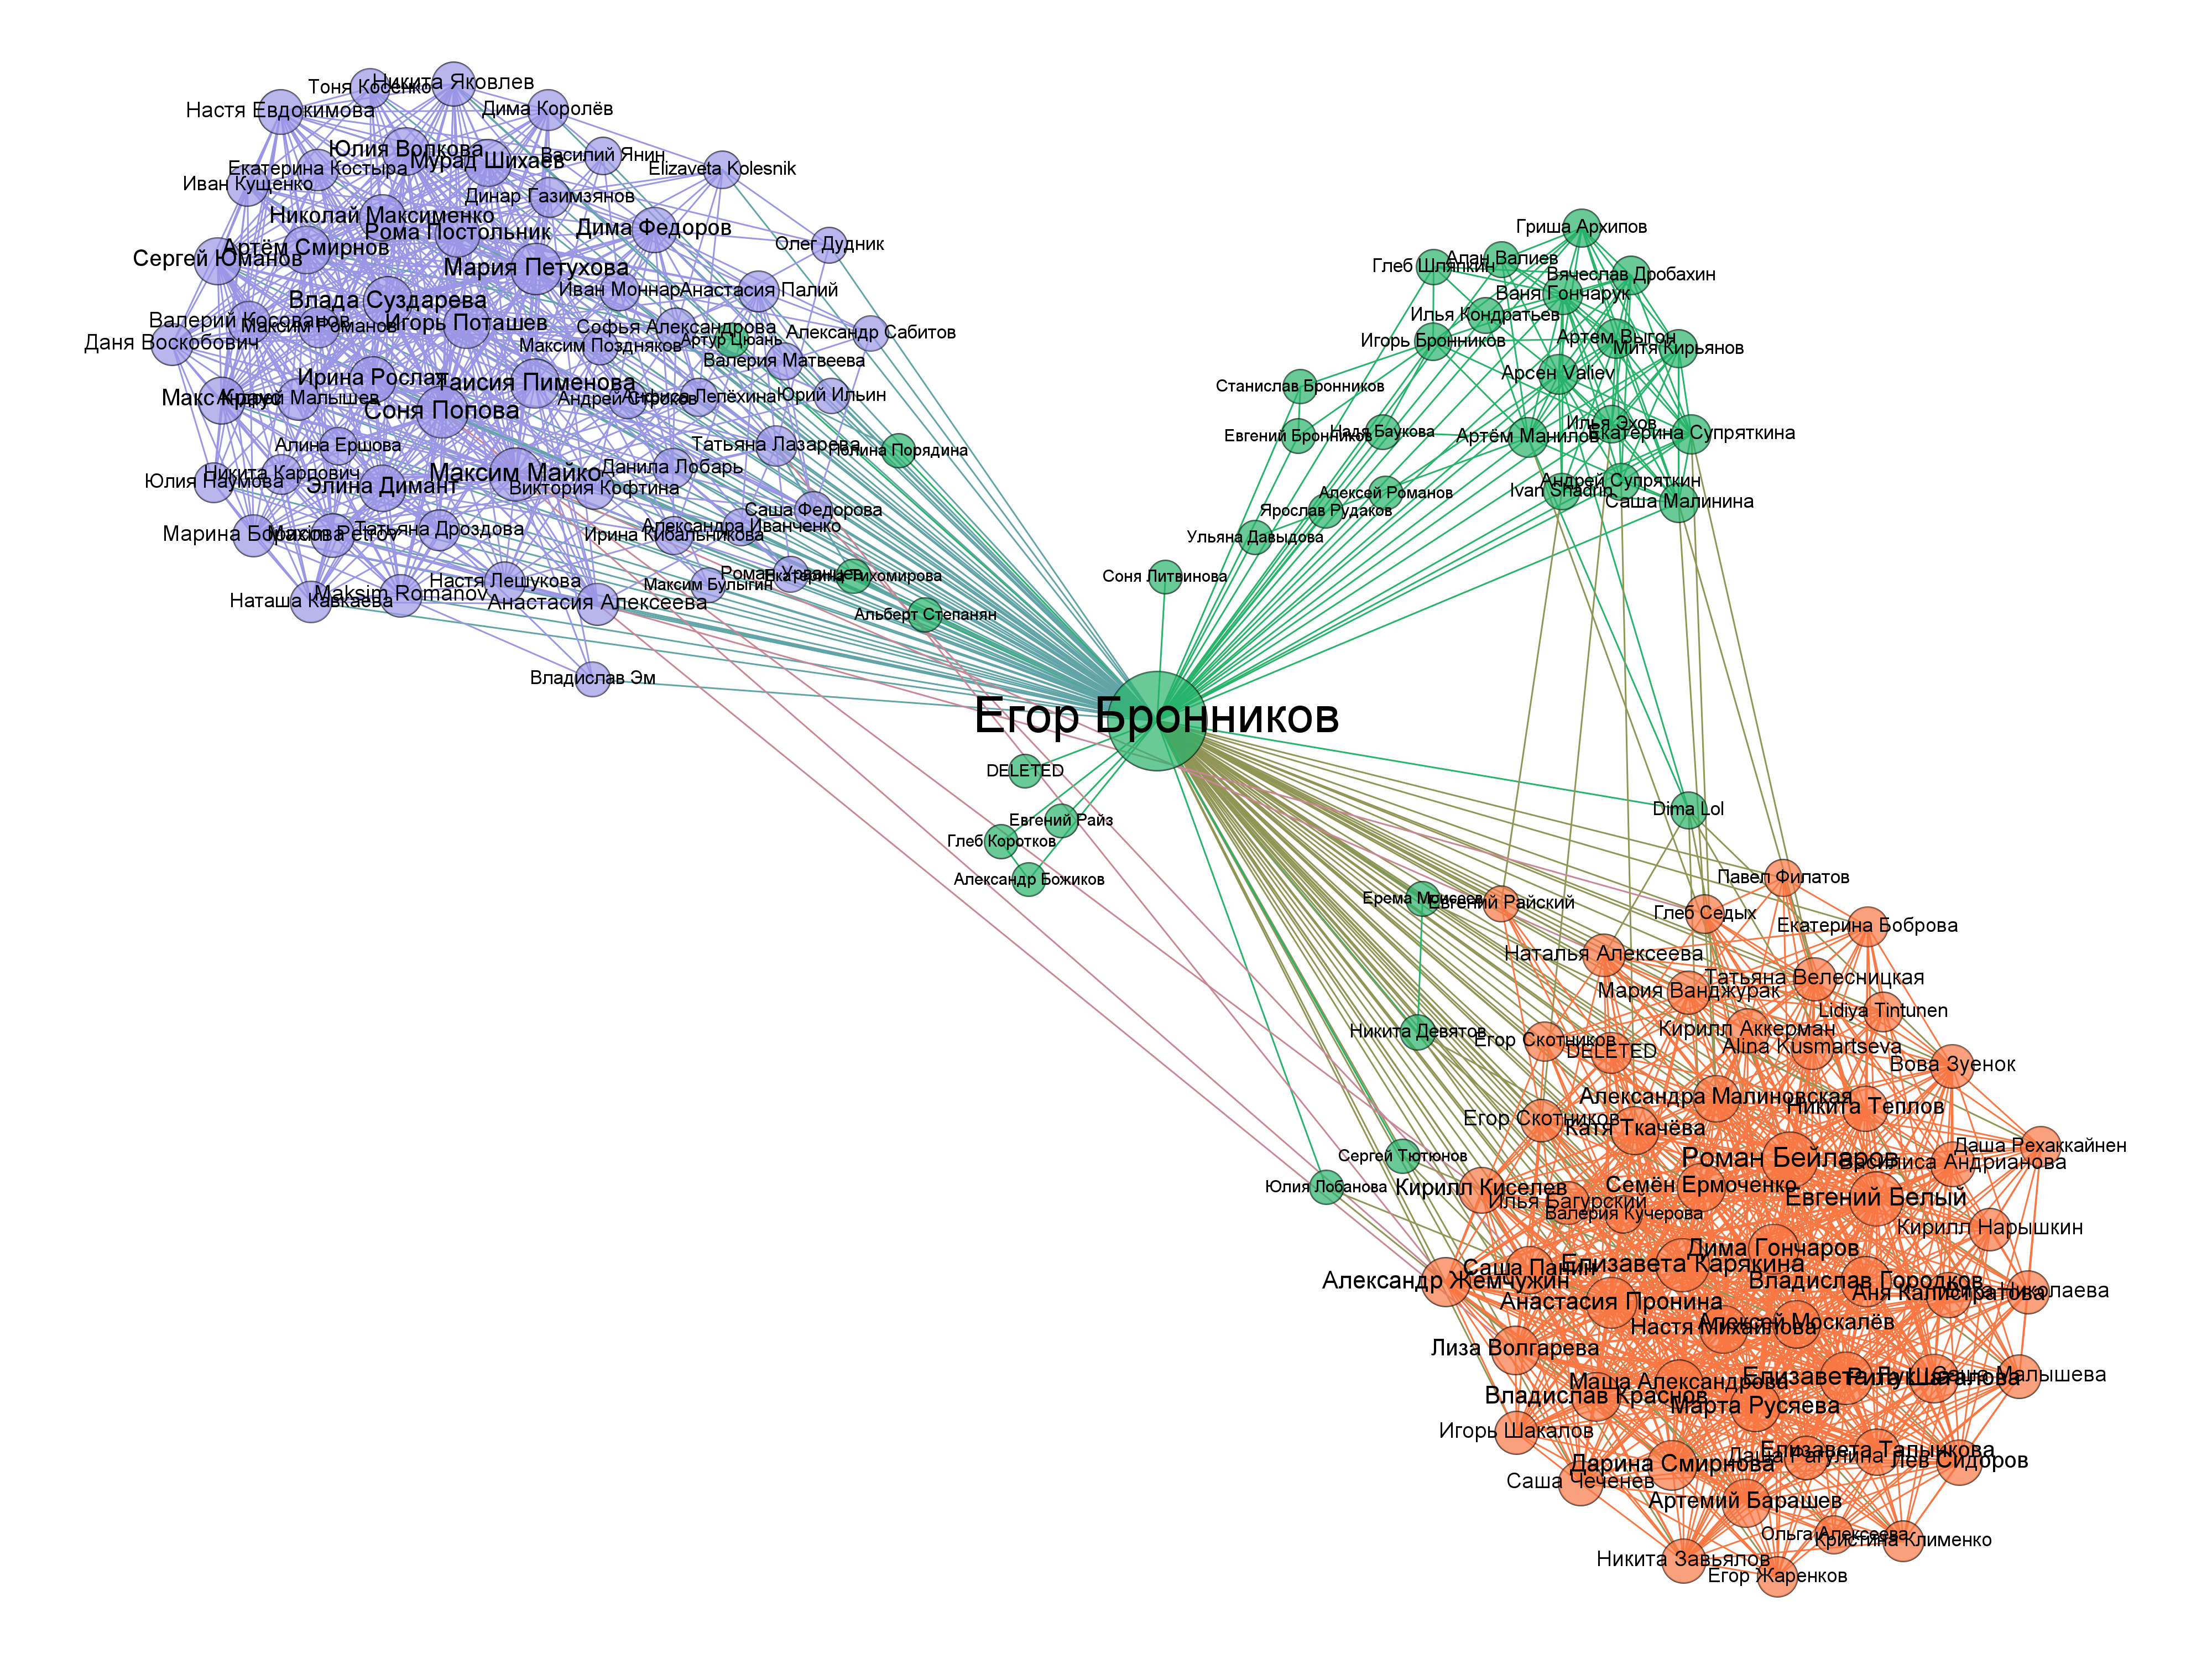
\includegraphics[width=9cm,height=7cm]{images/gephi}
        \end{center}
    \end{frame}
    
    % 7 слайд
    \begin{frame}
		\frametitle{Сбор данных и визуализация}
        \justifying
        Визуализация данных с помощью модуля \textit{NetworkX}.
        \begin{center}
            \includegraphics[width=7cm,height=6cm]{images/networkx}
        \end{center}
    \end{frame}

    \section{Характеристики сети}

    % 8 слайд
    \begin{frame}
		\frametitle{Характеристики сети}
        \vspace{-10pt}
        \begin{block}{Степень связности}
            \justifying
            В метрике степени связности важность вершины определяется тем, с каким количеством смежных вершин она связана.
            \[ deg(i) = \sum_{j \in V}m_{ij} \]
        \end{block}
        \vfill\pause
        \begin{block}{Степень близости у другим узлам}
            \justifying
            Степень близости к другим узлам можно определить как то, насколько близко к определённому субъекту находятся другие субъекты сети.
            \[ C(i) = \sum_{j \in V}d_{ij} \]
            где $d_{ij} -$ количество звеньев в кратчайшем пути от вершины $i$ до вершины $j$.
        \end{block}
        \tableofcontents[part=3, pausesections]
	\end{frame}

    % 9 слайд
    \begin{frame}
        \frametitle{Характеристики сети}
        \vspace{-10pt}
        \begin{block}{Степень посредничества}
            \justifying
            Степень посредничества представляет собой количество раз, которое участник должен пройти через данный узел, чтобы достичь другого участника сети.
            \[ b(i) = \sum_{j,k \in V} \dfrac{g_{ijk}}{g_{jk}} \]
            где $g_{jk} -$ это количество кратчайших путей от вершины $j$ до вершины $k$;\\
            $g_{ijk} -$ это количество кратчайших путей от вершины $j$ до вершины $k$ проходящих через вершину $i$.
        \end{block}
        \pause
        \vspace{-5pt}
        \begin{block}{Эксцентриситет}
            \justifying
            \[ E(i) = \max_{j \in V}d_{ij} \]
            где $d_{ij} -$ количество звеньев в кратчайшем пути от вершины $i$ до вершины $j$.
        \end{block}
    \end{frame}
    
    \section{Генетический алгоритм}

    % 10 слайд
    \begin{frame}
		\frametitle{Генетический алгоритм}
        \tableofcontents[part=4, pausesections]
        Пусть $S=(I,J)$ подматрица матрицы $A$, где $I -$ это подмножество строк $X = \{I_1, \dots, I_N\}$ матрицы $A$ и $J -$ это подмножество столбцов $Y = \{J_1, \dots, J_N\}$ матрицы $A$.
        \begin{block}{Постановка задачи}
            \justifying
            Найти разбиение матрицы смежности $A$ на $k$ подматриц, которые максимизируют сумму плотностей подматриц.
        \end{block}
	\end{frame}

    % 11 слайд
    \begin{frame}
		\frametitle{Генетический алгоритм}
        \vspace{-10pt}
        \begin{block}{Среднее значение строки}
        Пусть $a_{iJ}$ означает среднее значение $i$-й строки $S$:
            \[ a_{iJ} = \dfrac{1}{|J|}\sum_{j \in J} a_{ij} \]
        \end{block}
        \begin{block}{Среднее значение столбца}
        Пусть $a_{Ij}$ означает среднее значение $j$-й столбца $S$:
            \[ a_{Ij} = \dfrac{1}{|I|}\sum_{i \in I} a_{ij} \]
        \end{block}
        \begin{block}{Объём матрицы}
            \[ v_{S} = \sum_{i \in I, j \in J} a_{ij} \]
        \end{block}
    \end{frame}
    
    % 12 слайд
    \begin{frame}
		\frametitle{Генетический алгоритм}
        \begin{block}{Среднее значение мощности подматрицы}
            Среднее значение мощности подматрицы $S$ порядка $r$, обозначаемое как $M(S)$, рассчитывается по следующей формуле:
            \[ M(S) = \dfrac{\sum_{i \in I}(a_{iJ})^r}{|I|}\]
        \end{block}
        \begin{block}{Оценка множества разбиений}
            Оценка множества разбиений $\{S_1, \dots, S_k\}$ матрицы $A$ определяется следующим образом:
            \[ CS = \sum_{i=1}^{k} Q(S_i) \longrightarrow \max \]
            где оценка подматрицы $S_i$ определяется как: $Q(S_i) = M(S_i) \times v_{S_i}$
        \end{block}
    \end{frame}
    
    % 13 слайд
    \begin{frame}
		\frametitle{Генетический алгоритм}
        \begin{center}
            \includegraphics[width=313px,height=211px]{images/galgorithm}
        \end{center}
    \end{frame}

    % 14 слайд
    \begin{frame}
        \frametitle{Генетический алгоритм}
        \begin{block}{Инициализация}
            \justifying
            Инициализация индивидов популяции осуществляется следующим образом:
            \vspace{-0.5cm}
            \begin{center}
                \includegraphics[width=170px,height=35px]{images/init}
            \end{center}
        \end{block}
        \pause
        \begin{block}{Создание решений задачи}
            \begin{enumerate}
                \item генерируется исходный список подмножеств индивида как пара $\{\{i, g_i\} \; | \; \forall i \in \{1, \dots, N\}\}$;
                \item два подмножества объединяются если существует элемент из пересечения этих разбиений.
            \end{enumerate}
        \end{block}
    \end{frame}

    % 15 слайд
    \begin{frame}
		\frametitle{Генетический алгоритм}
        \begin{center}
            \includegraphics[width=313px,height=211px]{images/selection}
        \end{center}
    \end{frame}
    
    % 16 слайд
    \begin{frame}
		\frametitle{Генетический алгоритм}
        \begin{center}
            \includegraphics[width=313px,height=211px]{images/crossover}
        \end{center}
    \end{frame}
    
    % 17 слайд
    \begin{frame}
		\frametitle{Генетический алгоритм}
        \begin{center}
            \includegraphics[width=313px,height=211px]{images/mutation}
        \end{center}
    \end{frame}
    
    % 18 слайд
    \begin{frame}
		\frametitle{Генетический алгоритм}
        Визуализация полученного результата:
        \begin{center}
            \includegraphics[width=160px,height=200px]{images/ga_results}
        \end{center}
    \end{frame}
    
    \section{Алгоритм Гирван-Ньюмена}

    % 19 слайд
    \begin{frame}
		\frametitle{Алгоритм Гирван-Ньюмена}
        \vspace{-12pt}
        \begin{block}{Степень посредничества ребра}
            \justifying
            \[ c_B(e) = \sum_{s \in V, t \in V} \dfrac{\sigma(s,t|e)}{\sigma(s,t)}\]
            где $\sigma(s, t) -$ количество кратчайших путей между вершинами $s$ и $t$;\\
            $\sigma(s,t|e) -$ количество кратчайших путей между вершинами $s$ и $t$, которые проходят через ребро $e$\\
        \end{block}
        \vspace{-6pt}
        \pause
        \begin{block}{Модулярность}
            \justifying
            \[ Q = \sum_{c=1}^n \left[\dfrac{L_c}{m}-\gamma\left(\dfrac{k_c}{2m}\right)^2\right] \]
            где $m$ $-$ количество рёбер;\\
            $c$ $-$ сообщество;\\
            $L_c$ $-$ количество внутренних рёбер сообщества $c$;\\
            $k_c$ $-$ сумма степеней вершин в сообществе $c$;\\
            $\gamma$ $-$ параметр разрешения.
        \end{block}
        \tableofcontents[part=5, pausesections]
    \end{frame}
    
    % 20 слайд
    \begin{frame}
		\frametitle{Алгоритм Гирван-Ньюмена}
        \begin{block}{Описание алгоритма}
            \justifying
            Данный алгоритм может быть сформулирован несколькими следующими этапами:
            \begin{enumerate}
                \item вычисляются степени посредничества всех рёбер;
                \item ребро с наибольшей степенью посредничества удаляется;
                \item степени посредничества всех затронутых рёбер вычисляются заново;
                \item шаги 2 и 3 повторяются до тех пор, пока уровень модулярности не станет убывать.
            \end{enumerate}
        \end{block}
    \end{frame}
    
    % 21 слайд
    \begin{frame}
		\frametitle{Алгоритм Гирван-Ньюмена}
        Визуализация полученного результата:
        \begin{center}
            \includegraphics[width=160px,height=200px]{images/gn_results}
        \end{center}
    \end{frame}
    
    \section{Заключение}

    % 22 слайд
    \begin{frame}
		\frametitle{Заключение}
        \tableofcontents[part=6, pausesections]
        В ходе прохождения учебной практики, посвящённой приобретению навыков научно-исследовательской работы были достигнуты следующие результаты:
        \begin{itemize}
            \item проанализированы метрики и характеристики социальных графов;
            \item реализованы два алгоритма нахождения сообществ;
            \item изучены вспомогательные средства для визуализации графов.
        \end{itemize}
        \begin{figure}[ht]
        \begin{minipage}[b]{0.45\linewidth}
            \centering
            \includegraphics[width=140px]{images/ga_results2}
            \caption*{\textit{Генетический алгоритм}}
        \end{minipage}
        \hspace{0.5cm}
        \begin{minipage}[b]{0.45\linewidth}
            \centering
            \includegraphics[width=140px]{images/gn_results2}
            \caption*{\textit{Алгоритм Гирван-Ньюмена}}
        \end{minipage}
    \end{figure}
    \end{frame}
\end{document}
